% Ploicy Gradient method in Evolutionary Pricing Games
\documentclass[a4paper,12pt]{article}  %% important: a4paper first

\usepackage{graphicx}
\graphicspath{{./img/}}
\usepackage[notcite,notref]{showkeys}
\pdfoutput=1
\usepackage{natbib} 
\usepackage{amsthm}
\usepackage{newpxtext,newpxmath} 
\usepackage{microtype}
\linespread{1.10}        % Palatino needs more leading (space between lines)
\usepackage{xcolor}
\usepackage{pict2e} 

\usepackage{tikz} 
\usetikzlibrary{shapes}
\usetikzlibrary{arrows.meta}

%\usepackage{smallsec}
\usepackage{graphicx}
%\usepackage[pdflatex]{hyperref}
\usepackage[hyphens]{url} 
\usepackage[colorlinks,linkcolor=purple,citecolor=blue]{hyperref}
%\usepackage{hyperref}
\urlstyle{sf}
\usepackage[format=hang,justification=justified,labelfont=bf,labelsep=quad]{caption} 
% \input macros-drawtree
\oddsidemargin=.46cm    % A4
\textwidth=15cm
\textheight=23.3cm
\topmargin=-1.3cm
\clubpenalty=10000
\widowpenalty=10000
\predisplaypenalty=1350
\sfcode`E=1000  % normal spacing if E followed by period, as in "EFCE."
\sfcode`P=1000  % normal spacing if P followed by period, as in "NP." 
\newdimen\einr
\einr1.7em
\newdimen\eeinr 
\eeinr 1.7\einr
\def\aabs#1{\par\hangafter=1\hangindent=\eeinr
	\noindent\hbox to\eeinr{\strut\hskip\einr#1\hfill}\ignorespaces}
\def\rmitem#1{\par\hangafter=1\hangindent=\einr
	\noindent\hbox to\einr{\ignorespaces#1\hfill}\ignorespaces} 
\newcommand\bullitem{\rmitem{\raise.17ex\hbox{\kern7pt\scriptsize$\bullet$}}} 
\def\subbull{\vskip-.8\parskip\aabs{\raise.2ex\hbox{\footnotesize$\circ$}}}
\let\sfield\mathcal
\newtheorem{theorem}{Theorem}
\newtheorem{corollary}[theorem]{Corollary}
\newtheorem{example}[theorem]{Example}
\newtheorem{lemma}[theorem]{Lemma}
\newtheorem{proposition}[theorem]{Proposition}
\theoremstyle{definition}
\newtheorem{remark}[theorem]{Remark}
\newtheorem{definition}[theorem]{Definition}
\def\reals{{\mathbb R}} 
\def\eps{\varepsilon}
\def\prob{\hbox{prob}}
\def\sign{\hbox{sign}}
\def\proof{\noindent{\em Proof.\enspace}}
\def\proofof#1{\noindent{\em Proof of #1.\enspace}}
\def\endproof{\hfill\strut\nobreak\hfill\tombstone\par\medbreak}
\def\tombstone{\hbox{\lower.4pt\vbox{\hrule\hbox{\vrule
				\kern7.6pt\vrule height7.6pt}\hrule}\kern.5pt}}
\def\eqalign#1{\,\vcenter{\openup.7ex\mathsurround=0pt
		\ialign{\strut\hfil$\displaystyle{##}$&$\displaystyle{{}##}$\hfil
			\crcr#1\crcr}}\,}
\def\zw#1\par{\vskip2ex{\textbf{#1}}\par\nobreak} 
\newdimen\pix  % bounding box height for eps files
\pix0.08ex
\newsavebox{\figA} 
\parindent0pt
\parskip1.3ex

\title{%
	Plicy Gradient methods in the Evolutionary Pricing Game
}

\author{
}

%\date{Febuary 6, 2012}
\date{\today
	\\[1ex]
}

\begin{document}
	\maketitle
	
	\begin{abstract}
		The deep reinforcement learning model of an agent in duopoly multi-round pricing game and applying policy gradient methods to find the optimal strategy. 
		
		% \noindent 
		% \textbf{ACM classification:} 
		% CCS
		% $\to$ Theory of computation
		% $\to$ Theory and algorithms for application domains
		% $\to$ Algorithmic game theory and mechanism design
		% $\to$ Solution concepts in game theory,
		% exact and approximate computation of equilibria,
		% representations of games and their complexity
		% 
		% 
		% \strut
		% 
		% \noindent 
		% \textbf{AMS subject classification:} 
		% 91A18  (Games in extensive form)
		% 
		% \strut
		% 
		% \noindent 
		% \textbf{JEL classification:} 
		% C72 (Noncooperative Games)
		% 
		% \strut
		% 
		% \noindent 
		% \textbf{Keywords:}
		% extensive game,
		% correlated equilibrium,
		% polynomial-time algorithm,
		% computational complexity.
		% 
	\end{abstract}
	
	\section{Policy Gradient methods}
	
	
	
	\begin{figure}[hbt]
		\centering
		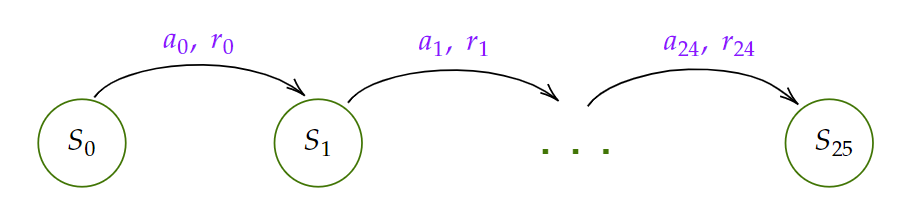
\includegraphics[width=11cm]{states_model}
		\caption{environment model}
		\label{f1equi}
	\end{figure}
	
	In \textit{action-value} methods such as Q-learning, the value of of each state or state-action pair is learned and based on these values, the policy would be determined.
	However, in \textit{Policy Gradient} methods, the policy is learnt directly without using value functions for action selection.
	
	
	Since the number of states in our model is large, we need a function approximator to parametrize the action preferences. We use a artificial neural network for this purpose and we show the vector of connection weights in our network as $ \theta $.
	
	The actions at each state are chosen in a way that action with higher valuation is more likely to be chosen. 
	
	\subsection{Action space} 
	
	The reward in each stage of the multi-round pricing game is determined by $ (D_i-P)\times(P-C) $ in which $ D_i $ is the agent's demand potential at the start of stage i and $ C $ is the agent's product cost. $ P^* = \frac{D_i + C}{2} $ maximises this quadratic concave function; we refer to $ P^* $ as \textit{myopic price} or \textit{monopoly price} at stage i. Playing the myopic price results in maximum payoff at the current stage but the demand potential for the next round would be affected, meaning it does\textbf{ not} necessarily result in the maximum overall return.
	
	We considered actions as the value below the monopoly price that should be played, in order to attract more demand and consequently more reward in later stages. In our model the action-space is discrete. In each stage, action $ a \in \lbrace0, 1, ..., 19\rbrace $ with step$ =3 $ that means the price can be $ 0, 3, 6, ... ,$ or $57 $ units less than the stage's myopic price. 
	
	For example, for the low-cost player ( $ C=57 $), if $ D_i = 180 $ at the start of stage i and action $ a = 5 $:
	\begin{equation*}
		P^* = \frac{180 + 57}{2} = 118.5  \rightarrow P = P^*- ( a\times \text{step}) = 118.5 - 5\times 3 = 103.5 \\
	\end{equation*}

	The actions are determined by sampling from the probability distribution over the action space that is the output of neural network.
	
	\subsection{State representation}
	
	The state should provide all the information that is needed for making a decision at each state. 
	In our model, the state includes following :
	\begin{itemize}
		\item current stage of game 
		\item agent's current demand potential $ (d) $
		\item agent's price in the last stage
		\item adversary's price history (last 3 stages)
	\end{itemize}	
	
	
	\tikzset{every picture/.style={line width=0.75pt}} %set default line width to 0.75pt        
	
	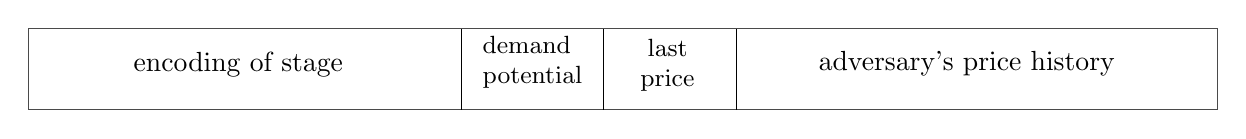
\begin{tikzpicture}[x=0.75pt,y=0.75pt,yscale=-1,xscale=1]
		%uncomment if require: \path (0,300); %set diagram left start at 0, and has height of 300
		
		%Shape: Rectangle [id:dp5062639226737371] 
		\draw  [color={rgb, 255:red, 74; green, 74; blue, 74 }  ,draw opacity=1 ] (53.4,101) -- (626.38,101) -- (626.38,140.24) -- (53.4,140.24) -- cycle ;
		%Straight Lines [id:da37083328217168265] 
		\draw    (262.06,101.39) -- (262.06,140.36) ;
		%Straight Lines [id:da032007577187648906] 
		\draw    (330.51,101.39) -- (330.51,140.36) ;
		%Straight Lines [id:da4042348455753717] 
		\draw    (394.55,101.39) -- (394.55,140.36) ;
		
		% Text Node
		\draw (102.95,111.47) node [anchor=north west][inner sep=0.75pt]  [font=\normalsize] [align=left] {encoding of stage};
		% Text Node
		\draw (271.06,103.39) node [anchor=north west][inner sep=0.75pt]  [font=\small] [align=left] {demand\\potential};
		% Text Node
		\draw (345,105) node [anchor=north west][inner sep=0.75pt]  [font=\small] [align=left] {\begin{minipage}[lt]{22.6pt}\setlength\topsep{0pt}
				\begin{center}
					last\\price
				\end{center}
				
		\end{minipage}};
		% Text Node
		\draw (433,111) node [anchor=north west][inner sep=0.75pt]  [color={rgb, 255:red, 0; green, 0; blue, 0 }  ,opacity=1 ] [align=left] {adversary's price history};
		
		
	\end{tikzpicture}
	
	\subsubsection{one-hot encoding of stage}
	\subsection{Structure of Neural Network}
	
	\subsection{Loss function}
	
	\subsection{Using Adam optimizer}
	
	
	\subsection{Structure of neural network}
	
	\section{Monte Carlo Policy Gradient}
	
	\section{Reinforcement with Baseline}
	
	\section{Actor-Critic method}
		
	

	
	%\bibliographystyle{ecta}
	%\bibliographystyle{acm}
	\small
	\bibliographystyle{book}
	\bibliography{bib-evol} 
	
\end{document}